\documentclass[tikz,border=7pt]{standalone}
\usepackage{amsmath}
\usepackage{pgfplots}
\pgfplotsset{compat=1.18}
\definecolor{ink}{HTML}{21352F}
\definecolor{teal}{HTML}{087F7B}
\definecolor{gold}{HTML}{C58B2A}
\definecolor{blue}{HTML}{4B77A8}
\definecolor{rose}{HTML}{B65A62}
\begin{document}
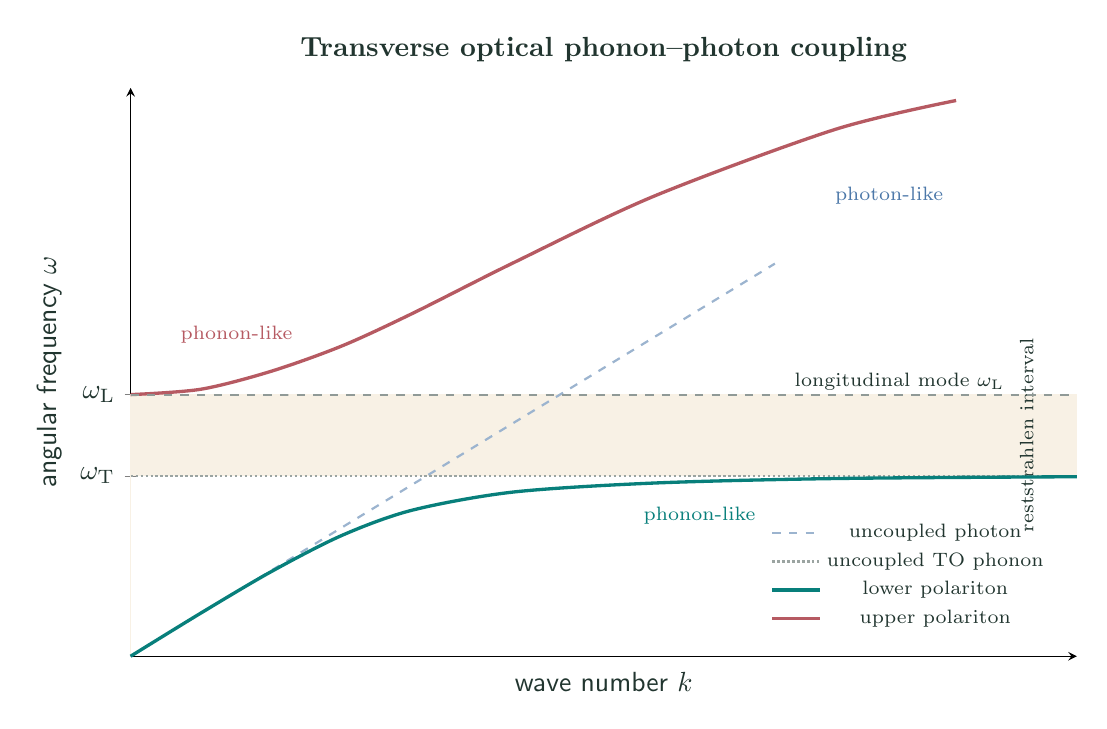
\begin{tikzpicture}[font=\sffamily,text=ink]
\begin{axis}[
  width=13.6cm,height=8.8cm,
  xmin=0,xmax=4.7,ymin=0,ymax=3.15,
  axis lines=left,xlabel={wave number $k$},ylabel={angular frequency $\omega$},
  xtick=\empty,ytick={1.0,1.45},yticklabels={$\omega_{\rm T}$,$\omega_{\rm L}$},
  title={Transverse optical phonon--photon coupling},title style={font=\bfseries},
  legend style={draw=none,fill=none,at={(0.98,0.03)},anchor=south east,font=\scriptsize},
  clip=false]
  \addplot[draw=gold!12,fill=gold!12,forget plot] coordinates {(0,1.0)(4.7,1.0)(4.7,1.45)(0,1.45)} \closedcycle;
  \node[font=\scriptsize,rotate=90] at (axis cs:4.45,1.225) {reststrahlen interval};
  \addplot[blue!55,dashed,thick,domain=0:3.2,samples=2] {0.68*x};
  \addlegendentry{uncoupled photon}
  \addplot[ink!45,densely dotted,thick,domain=0:4.7] {1.0};
  \addlegendentry{uncoupled TO phonon}
  \addplot[teal,very thick,smooth] coordinates {(0,0)(0.35,0.24)(0.7,0.47)(1.05,0.67)(1.4,0.81)(1.9,0.91)(2.6,0.96)(3.5,0.985)(4.7,0.995)};
  \addlegendentry{lower polariton}
  \addplot[rose,very thick,smooth] coordinates {(0,1.45)(0.35,1.48)(0.7,1.58)(1.05,1.72)(1.4,1.90)(1.9,2.18)(2.6,2.55)(3.5,2.92)(4.1,3.08)};
  \addlegendentry{upper polariton}
  \addplot[ink!50,dashed,thick,domain=0:4.7,forget plot] {1.45};
  \node[anchor=west,font=\scriptsize] at (axis cs:3.25,1.52) {longitudinal mode $\omega_{\rm L}$};
  \node[teal,anchor=west,font=\scriptsize] at (axis cs:2.5,0.78) {phonon-like};
  \node[rose,anchor=west,font=\scriptsize] at (axis cs:0.2,1.78) {phonon-like};
  \node[blue,anchor=west,font=\scriptsize] at (axis cs:3.45,2.55) {photon-like};
\end{axis}
\end{tikzpicture}
\end{document}
